\bbsection{Design Specifications}{design-specifications}

This section contains information regarding visual properties of certain UI elements. Examples of visual properties include height, width, and relative distance to another UI element. The UI elements highlighted in this section may range from text fields, to labels, or to switches and progress bars. \newline

Note that a light maroon line crossing right through the center of a parent UI element (e.g.: The Account Name table cell) indicates that it is divided into two equal portions. A darkened maroon line through a sub-element (e.g.: "Account Name" UI Label, "My Wallet" text field) indicates that it contains the property of being situated in the middle of the parent element. \newline

Note that a vertical or horizontal line leaning against the inner wall of a parent element indicates the distance between the sub-element to the parent element's walls. For example, in the figure below, it can be seen that the "Account Name" UI Label leans against the wall of its table cell, at a distance of zero points.

\bbsubsection{Add and Edit Account Screen}{add-and-edit-account-screen}
\centerline{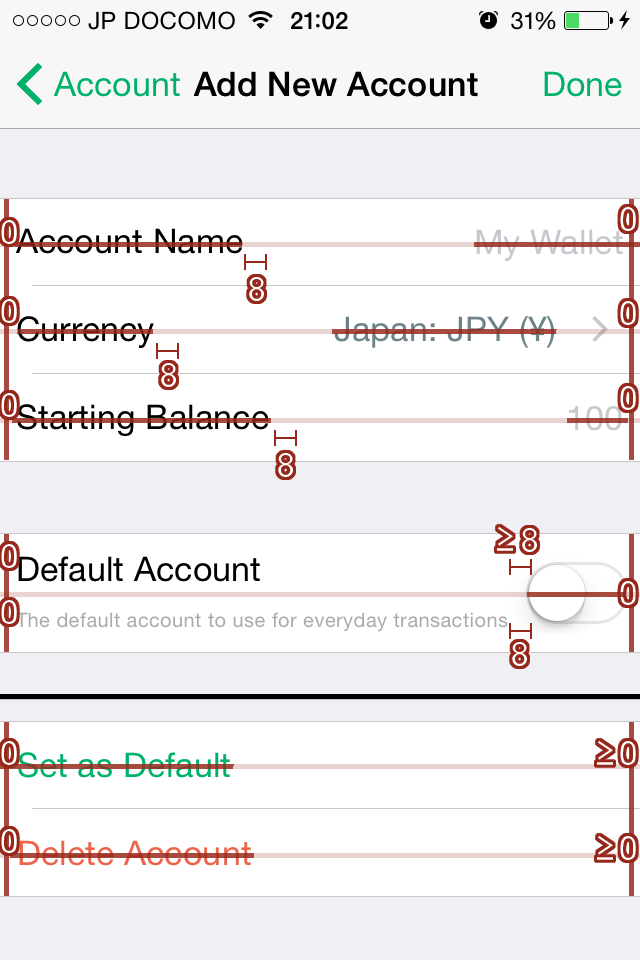
\includegraphics[scale=0.35]{ACC-0001-design}}